
\begin{figure}
\centering
\begin{subfigure}[b]{0.33\textwidth} 
  \centering 
  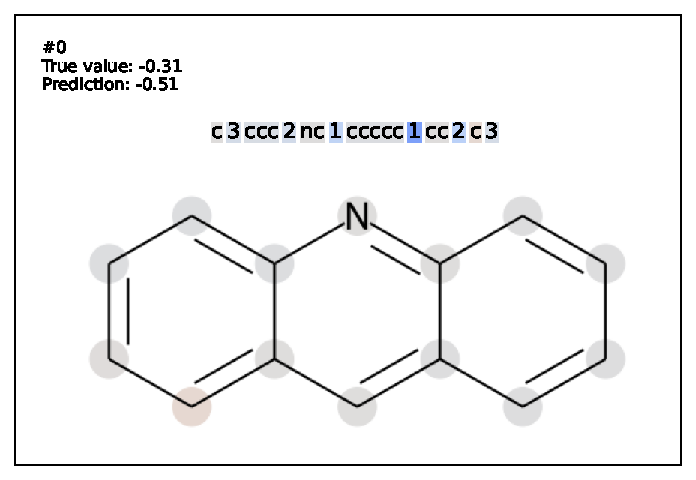
\includegraphics[width=\textwidth]{figures/esol/esol0.pdf} 
\end{subfigure}\begin{subfigure}[b]{0.33\textwidth} 
  \centering 
  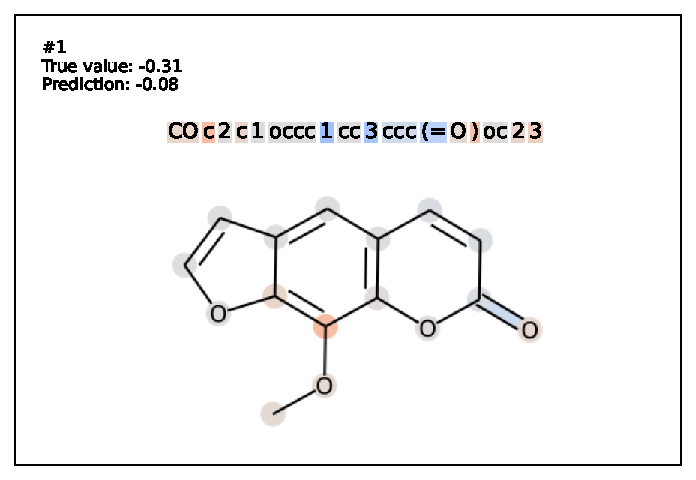
\includegraphics[width=\textwidth]{figures/esol/esol1.pdf} 
\end{subfigure}\begin{subfigure}[b]{0.33\textwidth} 
  \centering 
  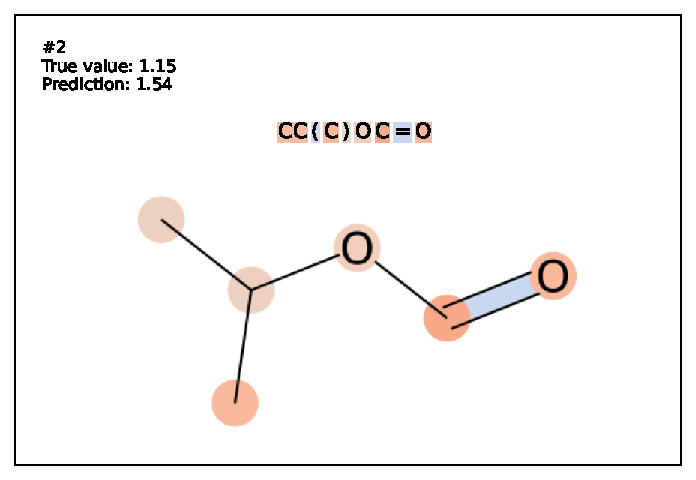
\includegraphics[width=\textwidth]{figures/esol/esol2.pdf} 
\end{subfigure}
\begin{subfigure}[b]{0.33\textwidth} 
  \centering 
  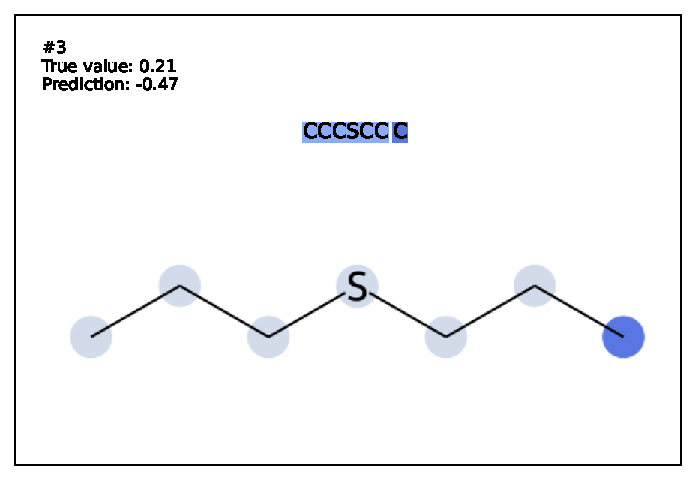
\includegraphics[width=\textwidth]{figures/esol/esol3.pdf} 
\end{subfigure}\begin{subfigure}[b]{0.33\textwidth} 
  \centering 
  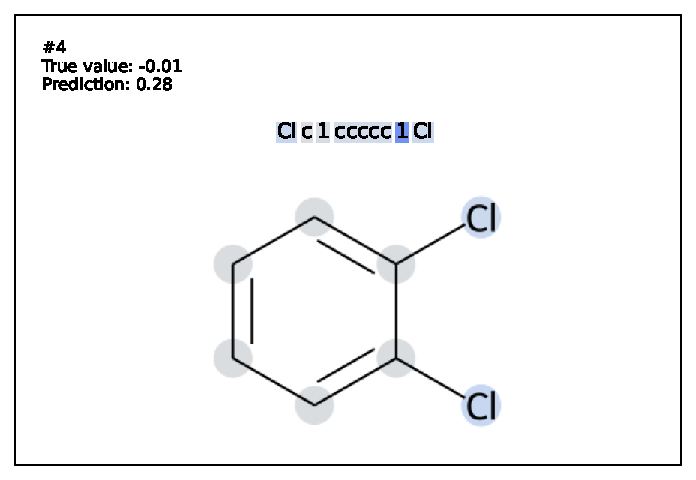
\includegraphics[width=\textwidth]{figures/esol/esol4.pdf} 
\end{subfigure}\begin{subfigure}[b]{0.33\textwidth} 
  \centering 
  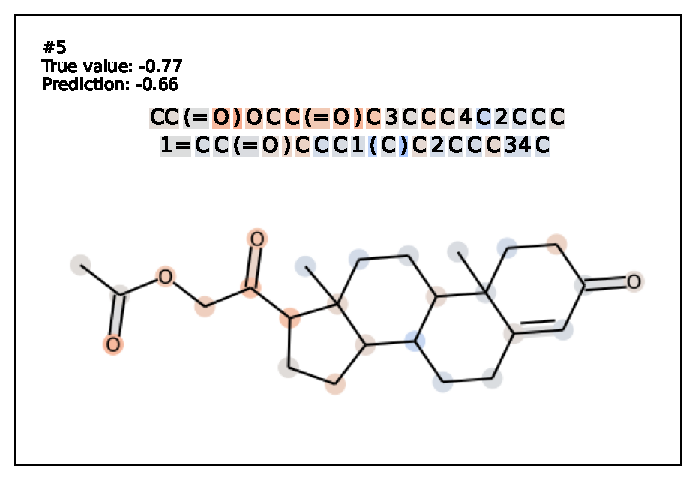
\includegraphics[width=\textwidth]{figures/esol/esol5.pdf} 
\end{subfigure}
\begin{subfigure}[b]{0.33\textwidth} 
  \centering 
  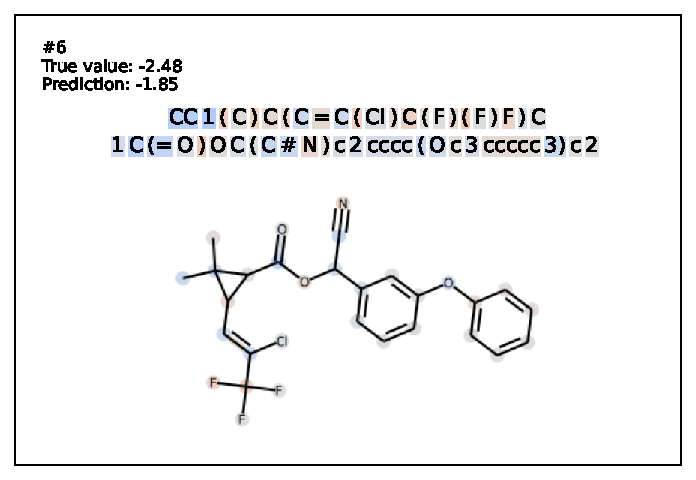
\includegraphics[width=\textwidth]{figures/esol/esol6.pdf} 
\end{subfigure}\begin{subfigure}[b]{0.33\textwidth} 
  \centering 
  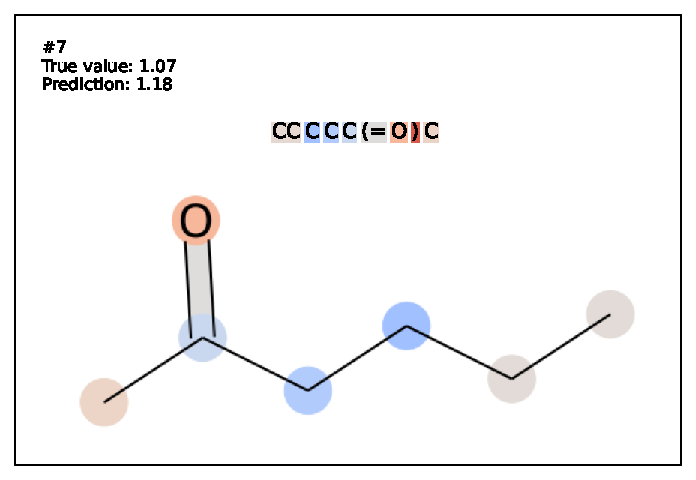
\includegraphics[width=\textwidth]{figures/esol/esol7.pdf} 
\end{subfigure}\begin{subfigure}[b]{0.33\textwidth} 
  \centering 
  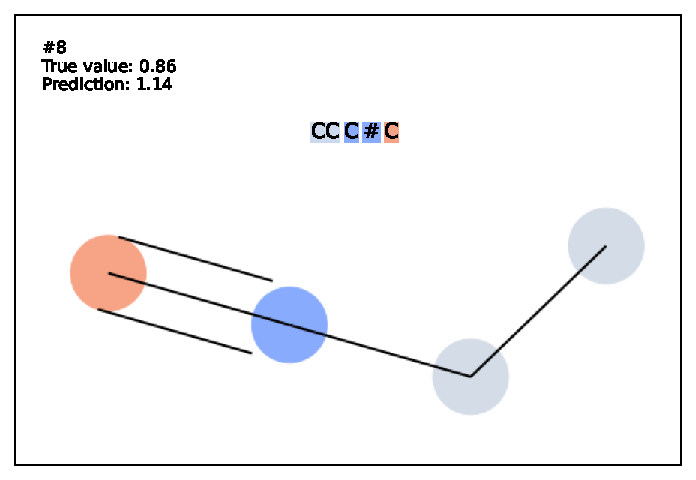
\includegraphics[width=\textwidth]{figures/esol/esol8.pdf} 
\end{subfigure}
\begin{subfigure}[b]{0.33\textwidth} 
  \centering 
  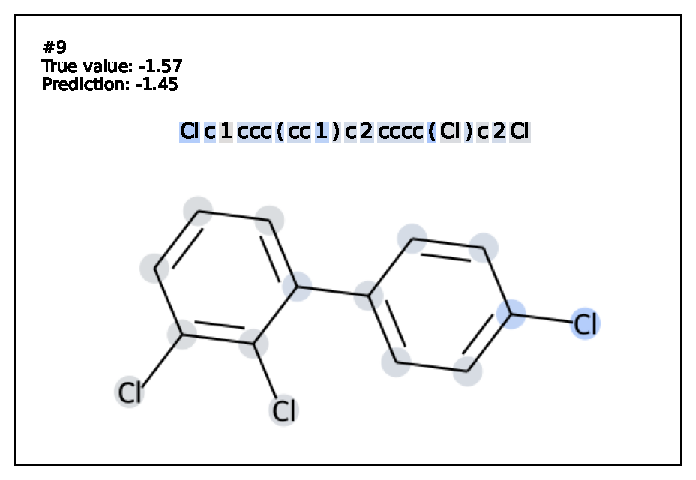
\includegraphics[width=\textwidth]{figures/esol/esol9.pdf} 
\end{subfigure}\begin{subfigure}[b]{0.33\textwidth} 
  \centering 
  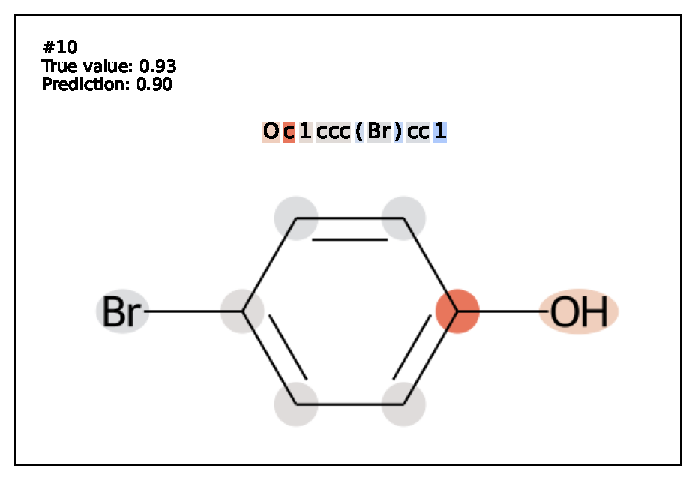
\includegraphics[width=\textwidth]{figures/esol/esol10.pdf} 
\end{subfigure}\begin{subfigure}[b]{0.33\textwidth} 
  \centering 
  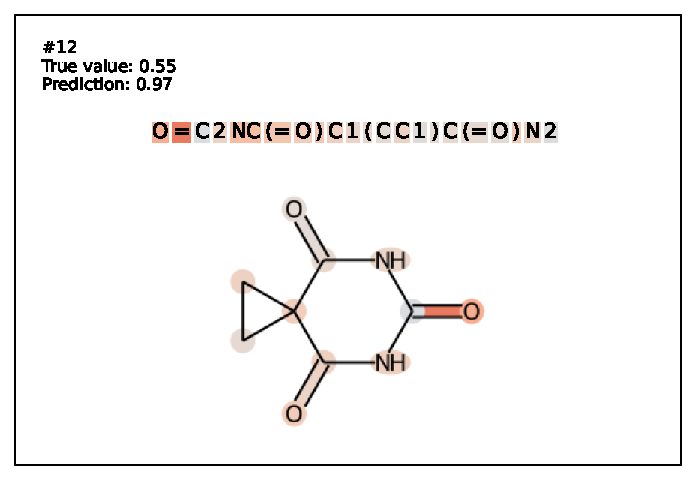
\includegraphics[width=\textwidth]{figures/esol/esol12.pdf} 
\end{subfigure}
\begin{subfigure}[b]{0.33\textwidth} 
  \centering 
  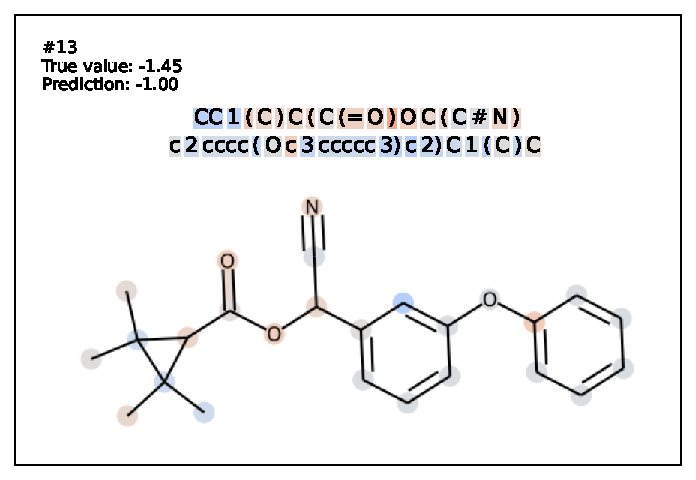
\includegraphics[width=\textwidth]{figures/esol/esol13.pdf} 
\end{subfigure}\begin{subfigure}[b]{0.33\textwidth} 
  \centering 
  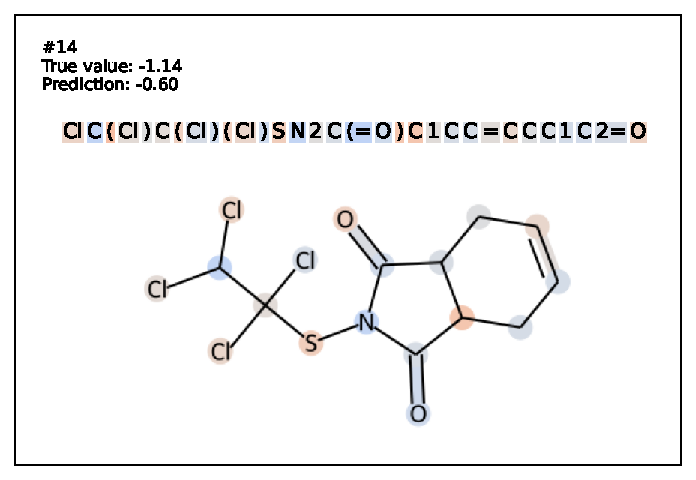
\includegraphics[width=\textwidth]{figures/esol/esol14.pdf} 
\end{subfigure}\begin{subfigure}[b]{0.33\textwidth} 
  \centering 
  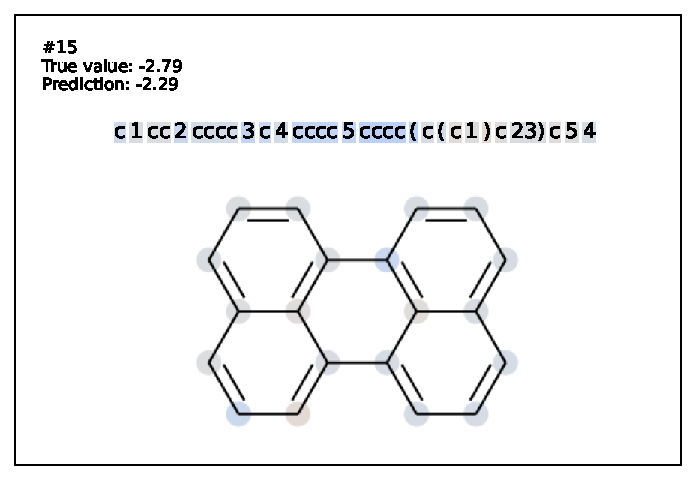
\includegraphics[width=\textwidth]{figures/esol/esol15.pdf} 
\end{subfigure}
\begin{subfigure}[b]{0.33\textwidth} 
  \centering 
  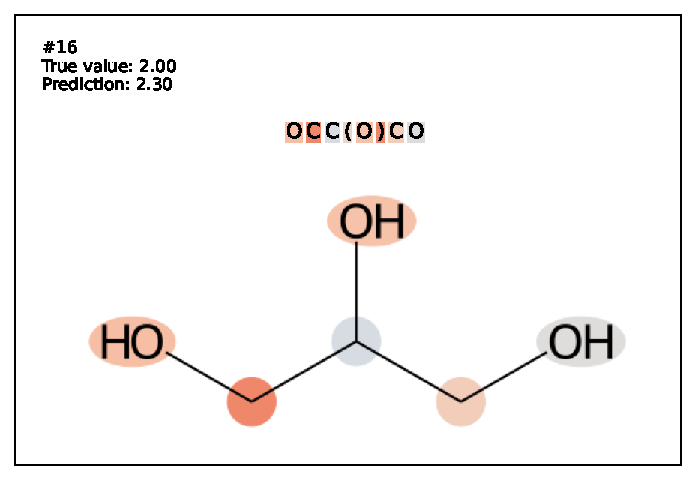
\includegraphics[width=\textwidth]{figures/esol/esol16.pdf} 
\end{subfigure}\begin{subfigure}[b]{0.33\textwidth} 
  \centering 
  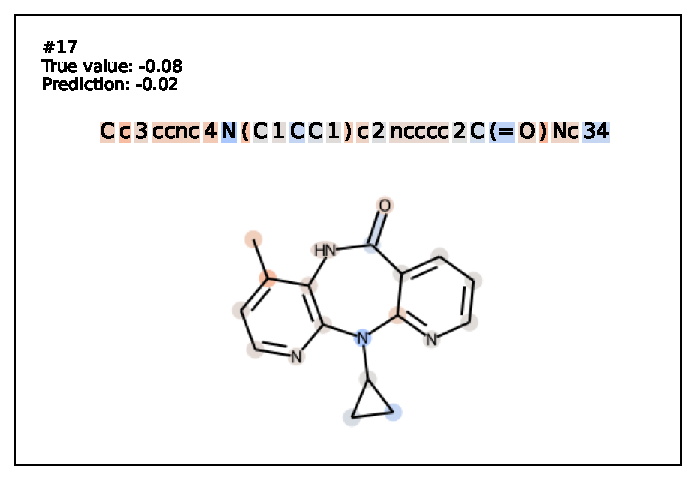
\includegraphics[width=\textwidth]{figures/esol/esol17.pdf} 
\end{subfigure}\begin{subfigure}[b]{0.33\textwidth} 
  \centering 
  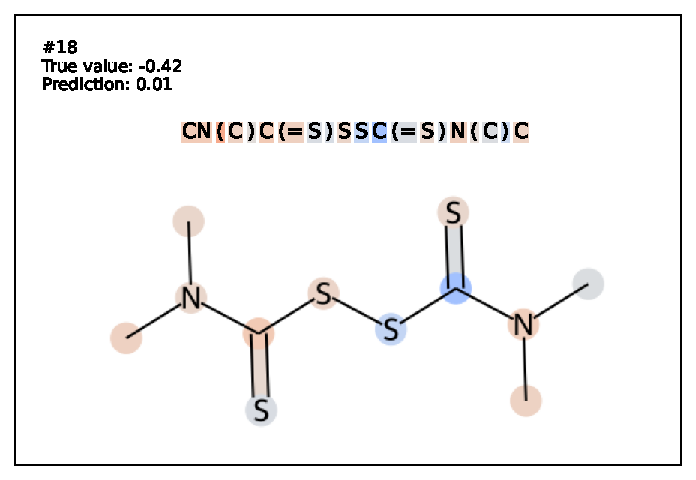
\includegraphics[width=\textwidth]{figures/esol/esol18.pdf} 
\end{subfigure}
\begin{subfigure}[b]{0.33\textwidth} 
  \centering 
  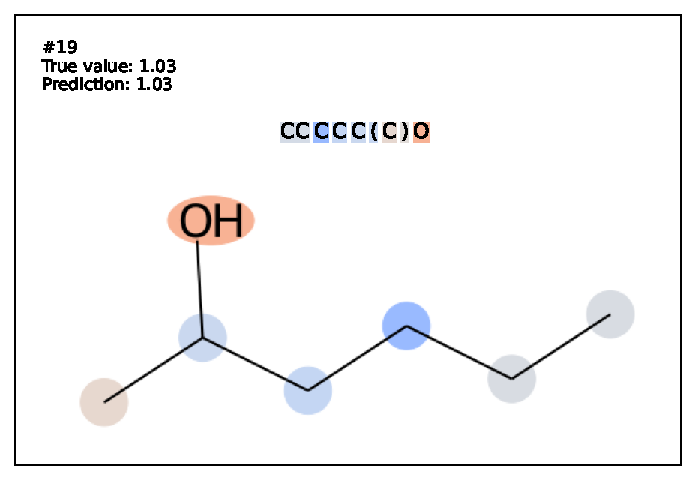
\includegraphics[width=\textwidth]{figures/esol/esol19.pdf} 
\end{subfigure}\begin{subfigure}[b]{0.33\textwidth} 
  \centering 
  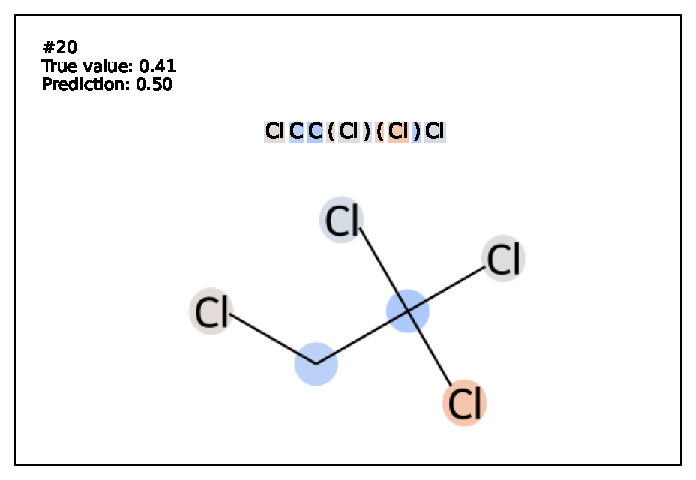
\includegraphics[width=\textwidth]{figures/esol/esol20.pdf} 
\end{subfigure}\begin{subfigure}[b]{0.33\textwidth} 
  \centering 
  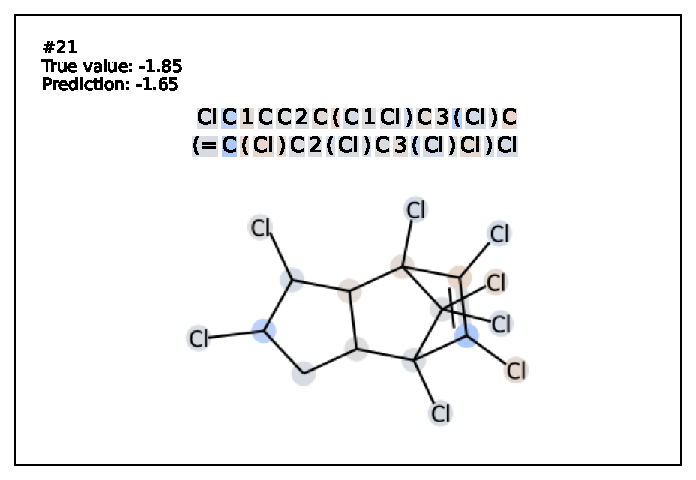
\includegraphics[width=\textwidth]{figures/esol/esol21.pdf} 
\end{subfigure}


\caption{Explaining predictions of the fine-tuned model on ESOL dataset. See Section \ref{sec:captum}. Part 1/3}
\label{fig:captum-esol-1}
\end{figure}




\begin{figure}
\centering

\begin{subfigure}[b]{0.33\textwidth} 
  \centering 
  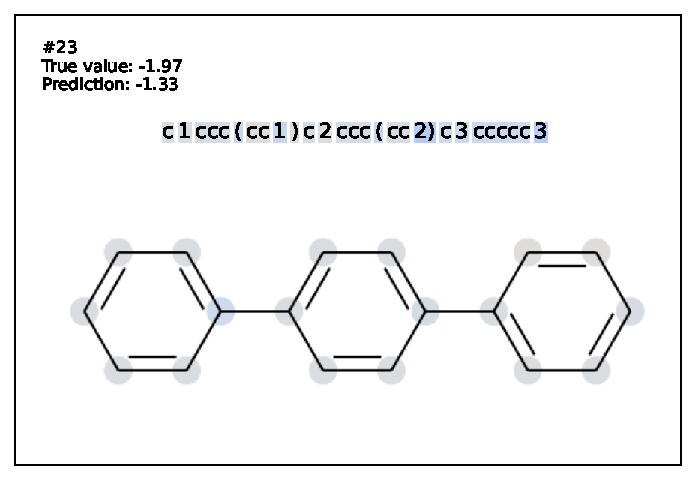
\includegraphics[width=\textwidth]{figures/esol/esol23.pdf} 
\end{subfigure}\begin{subfigure}[b]{0.33\textwidth} 
  \centering 
  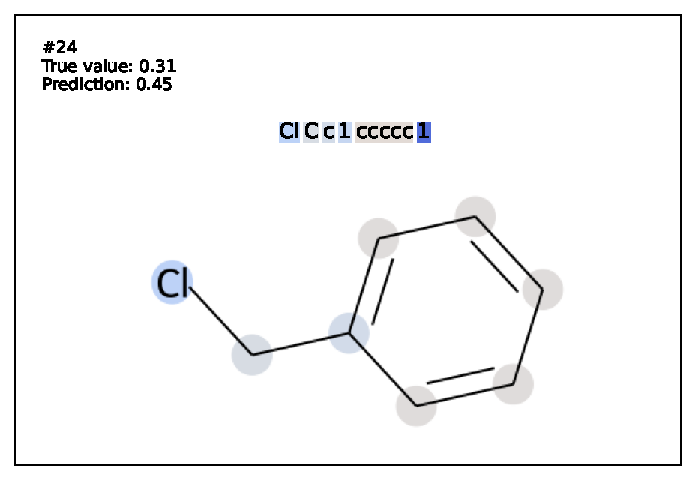
\includegraphics[width=\textwidth]{figures/esol/esol24.pdf} 
\end{subfigure}\begin{subfigure}[b]{0.33\textwidth} 
  \centering 
  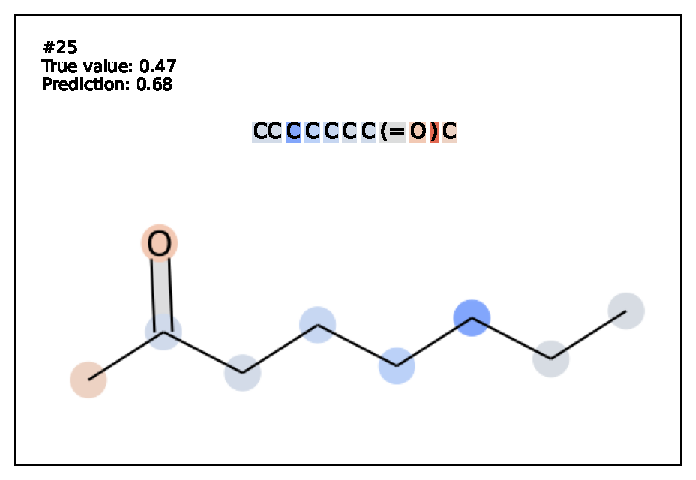
\includegraphics[width=\textwidth]{figures/esol/esol25.pdf} 
\end{subfigure}
\begin{subfigure}[b]{0.33\textwidth} 
  \centering 
  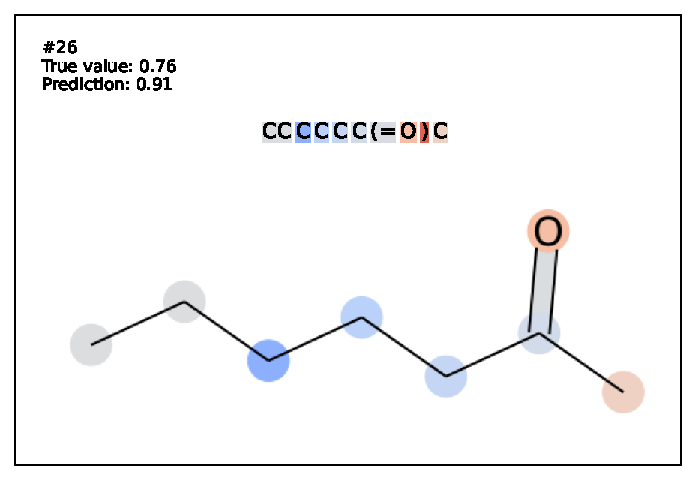
\includegraphics[width=\textwidth]{figures/esol/esol26.pdf} 
\end{subfigure}\begin{subfigure}[b]{0.33\textwidth} 
  \centering 
  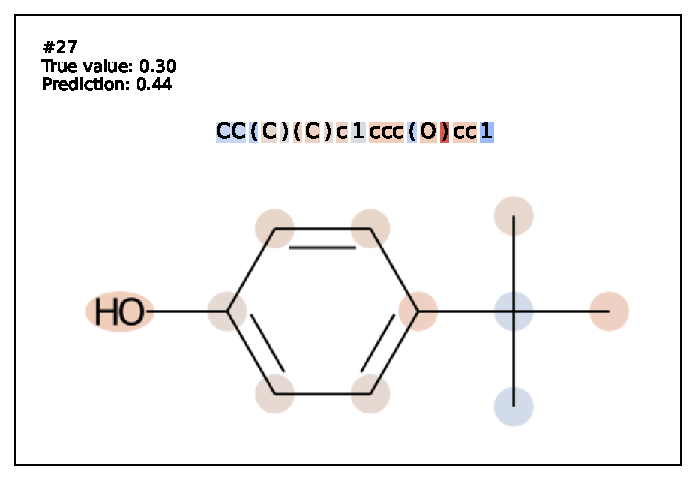
\includegraphics[width=\textwidth]{figures/esol/esol27.pdf} 
\end{subfigure}\begin{subfigure}[b]{0.33\textwidth} 
  \centering 
  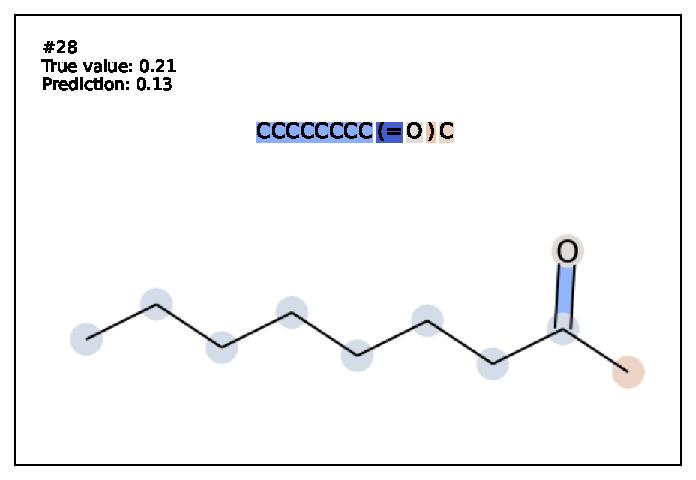
\includegraphics[width=\textwidth]{figures/esol/esol28.pdf} 
\end{subfigure}
\begin{subfigure}[b]{0.33\textwidth} 
  \centering 
  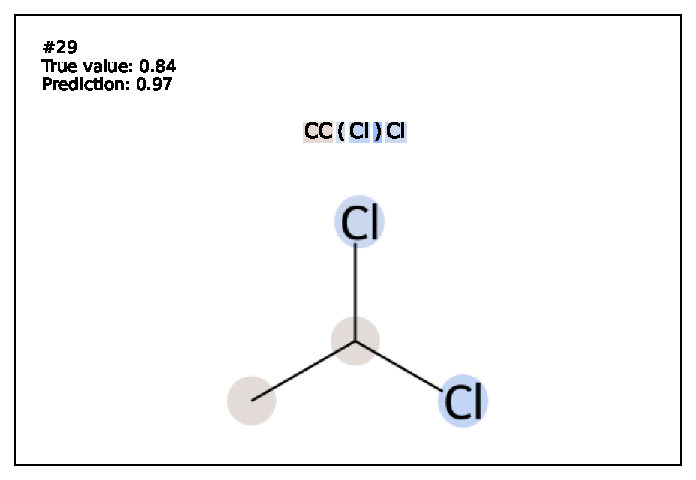
\includegraphics[width=\textwidth]{figures/esol/esol29.pdf} 
\end{subfigure}\begin{subfigure}[b]{0.33\textwidth} 
  \centering 
  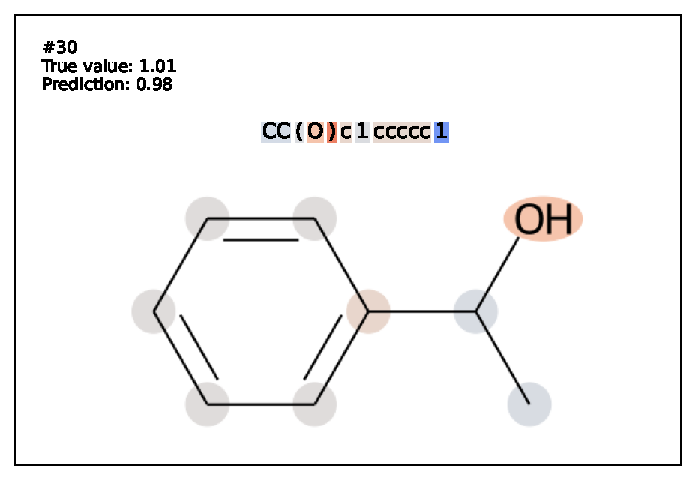
\includegraphics[width=\textwidth]{figures/esol/esol30.pdf} 
\end{subfigure}\begin{subfigure}[b]{0.33\textwidth} 
  \centering 
  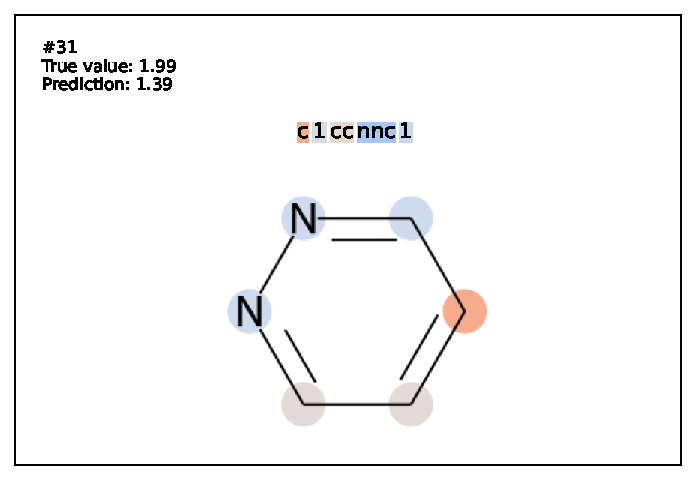
\includegraphics[width=\textwidth]{figures/esol/esol31.pdf} 
\end{subfigure}
\begin{subfigure}[b]{0.33\textwidth} 
  \centering 
  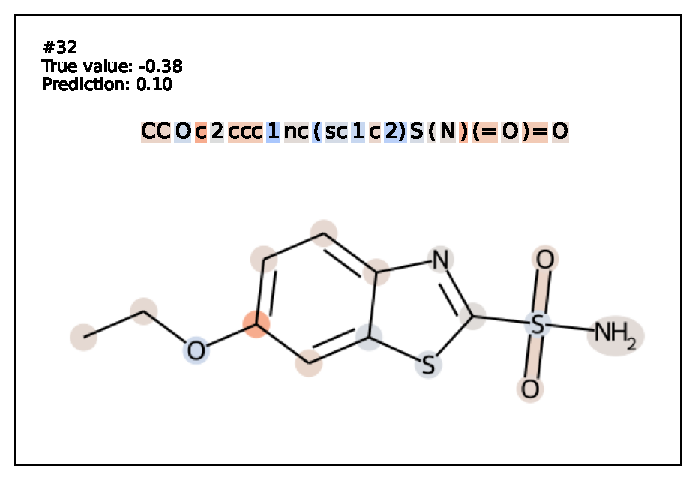
\includegraphics[width=\textwidth]{figures/esol/esol32.pdf} 
\end{subfigure}\begin{subfigure}[b]{0.33\textwidth} 
  \centering 
  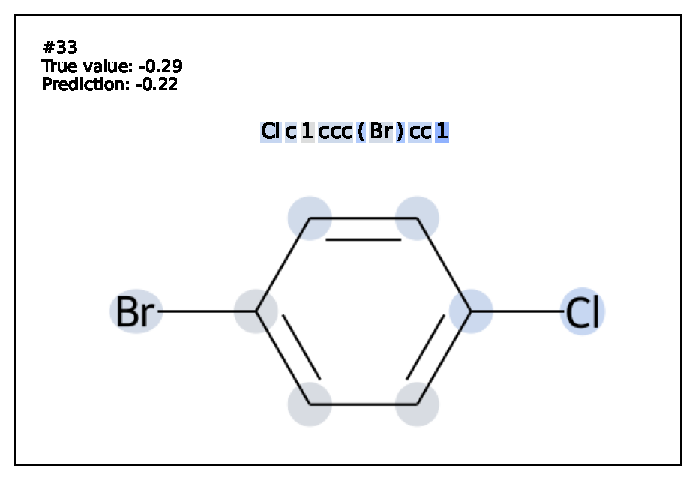
\includegraphics[width=\textwidth]{figures/esol/esol33.pdf} 
\end{subfigure}\begin{subfigure}[b]{0.33\textwidth} 
  \centering 
  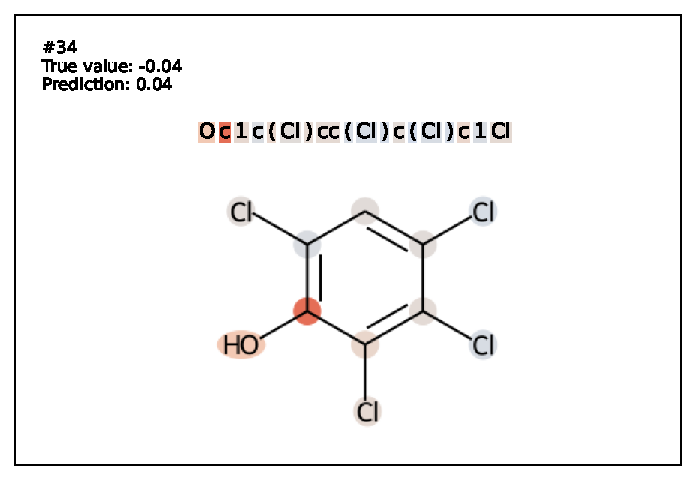
\includegraphics[width=\textwidth]{figures/esol/esol34.pdf} 
\end{subfigure}
\begin{subfigure}[b]{0.33\textwidth} 
  \centering 
  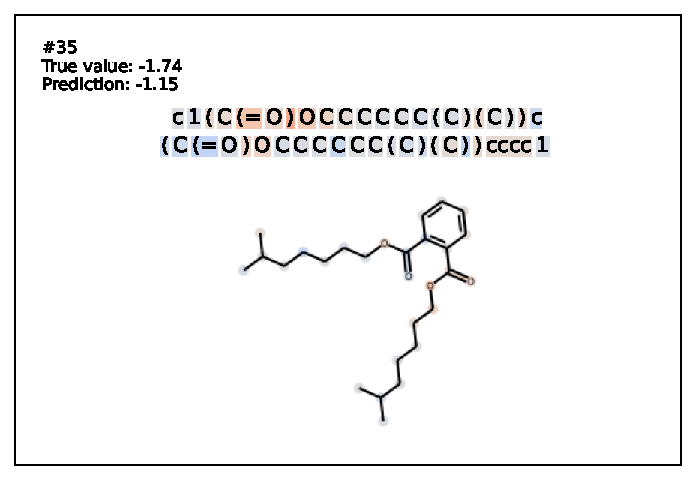
\includegraphics[width=\textwidth]{figures/esol/esol35.pdf} 
\end{subfigure}\begin{subfigure}[b]{0.33\textwidth} 
  \centering 
  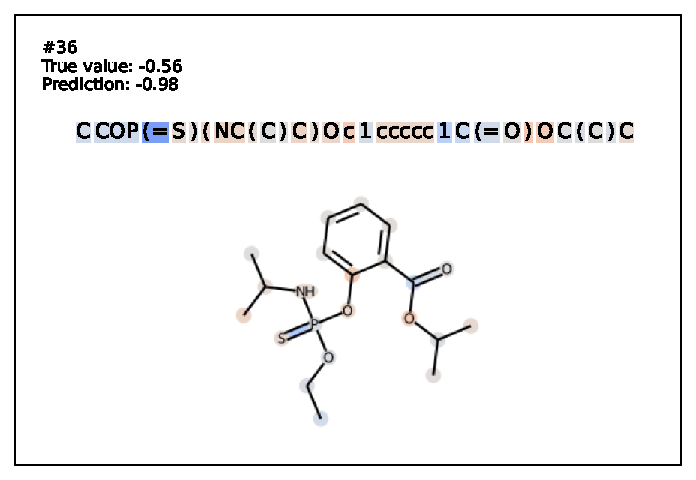
\includegraphics[width=\textwidth]{figures/esol/esol36.pdf} 
\end{subfigure}\begin{subfigure}[b]{0.33\textwidth} 
  \centering 
  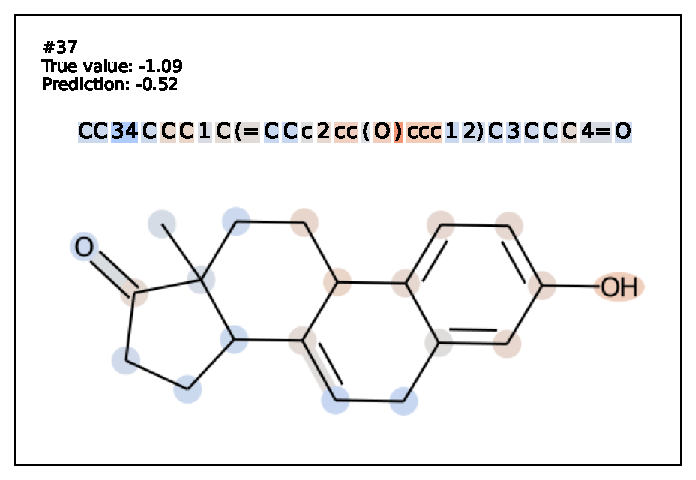
\includegraphics[width=\textwidth]{figures/esol/esol37.pdf} 
\end{subfigure}
\begin{subfigure}[b]{0.33\textwidth} 
  \centering 
  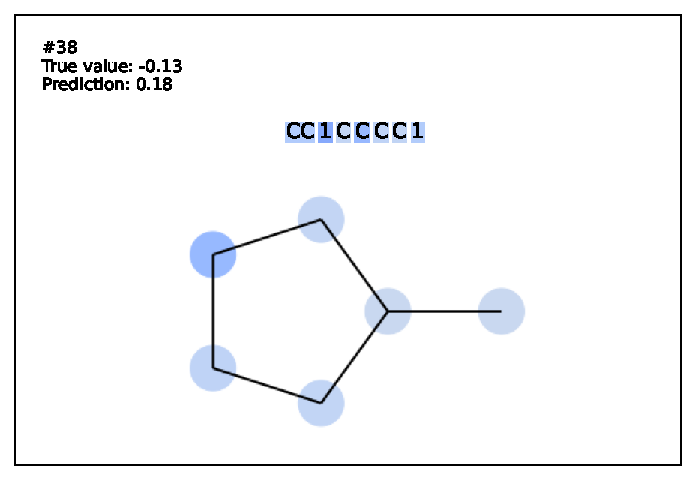
\includegraphics[width=\textwidth]{figures/esol/esol38.pdf} 
\end{subfigure}\begin{subfigure}[b]{0.33\textwidth} 
  \centering 
  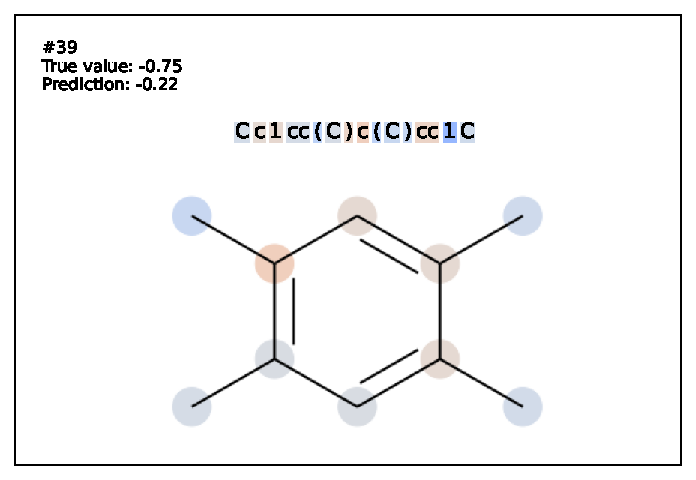
\includegraphics[width=\textwidth]{figures/esol/esol39.pdf} 
\end{subfigure}\begin{subfigure}[b]{0.33\textwidth} 
  \centering 
  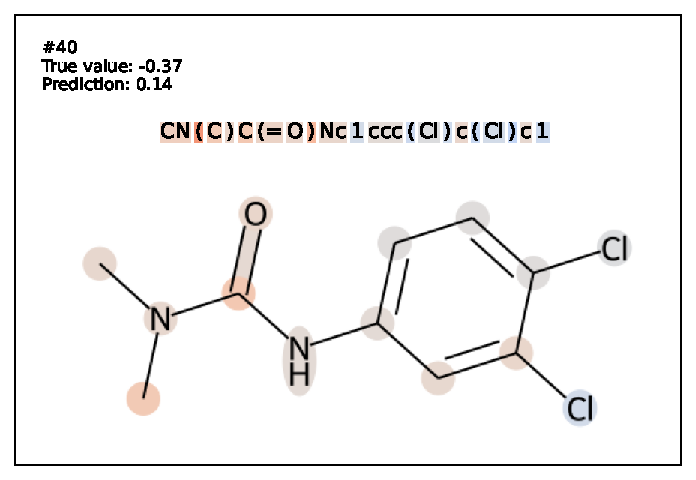
\includegraphics[width=\textwidth]{figures/esol/esol40.pdf} 
\end{subfigure}
\begin{subfigure}[b]{0.33\textwidth} 
  \centering 
  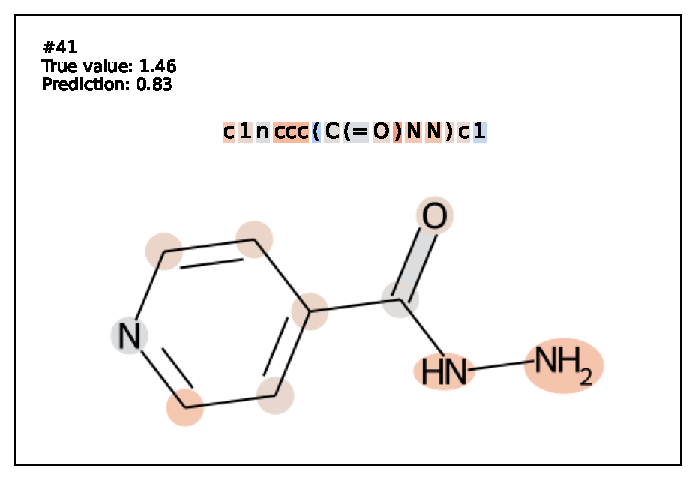
\includegraphics[width=\textwidth]{figures/esol/esol41.pdf} 
\end{subfigure}\begin{subfigure}[b]{0.33\textwidth} 
  \centering 
  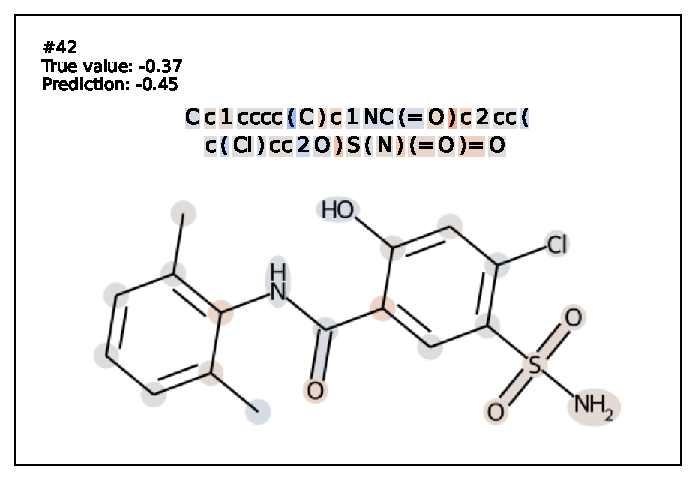
\includegraphics[width=\textwidth]{figures/esol/esol42.pdf} 
\end{subfigure}\begin{subfigure}[b]{0.33\textwidth} 
  \centering 
  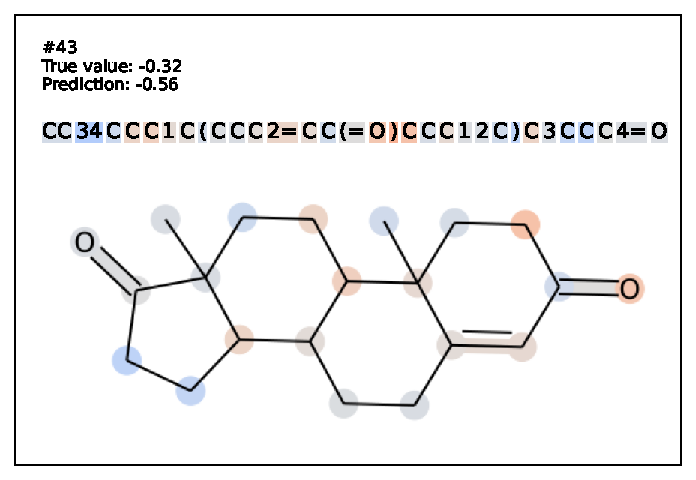
\includegraphics[width=\textwidth]{figures/esol/esol43.pdf} 
\end{subfigure}


\caption{Explaining predictions of the fine-tuned model on ESOL dataset. See Section \ref{sec:captum}. Part 2/3}
\label{fig:captum-esol-2}
\end{figure}




\begin{figure}[h]
\centering
\begin{subfigure}[b]{0.33\textwidth} 
  \centering 
  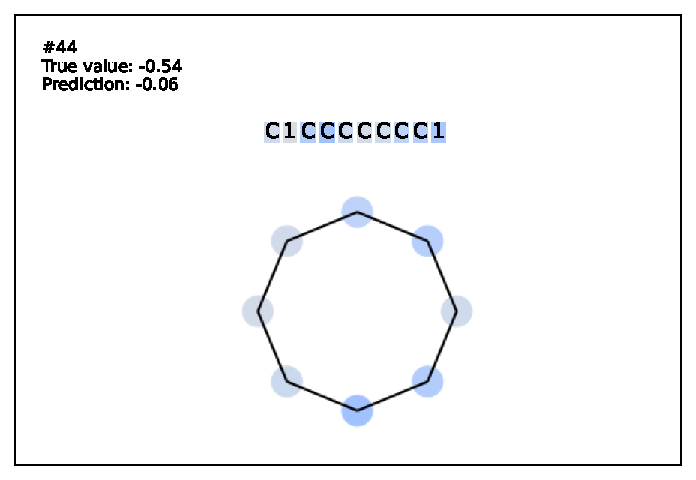
\includegraphics[width=\textwidth]{figures/esol/esol44.pdf} 
\end{subfigure}\begin{subfigure}[b]{0.33\textwidth} 
  \centering 
  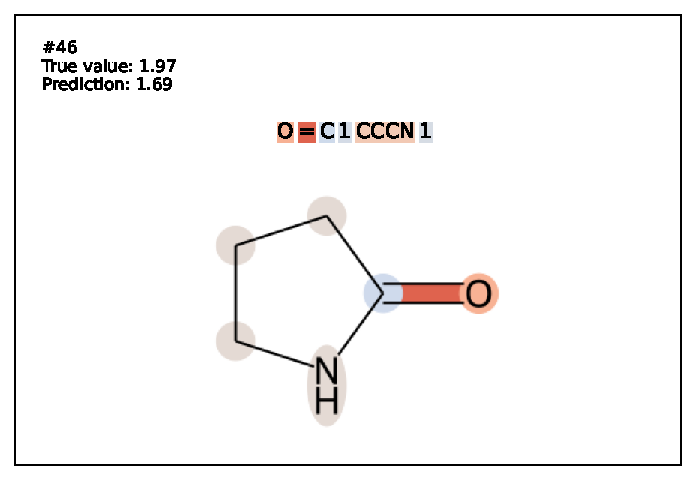
\includegraphics[width=\textwidth]{figures/esol/esol46.pdf} 
\end{subfigure}\begin{subfigure}[b]{0.33\textwidth} 
  \centering 
  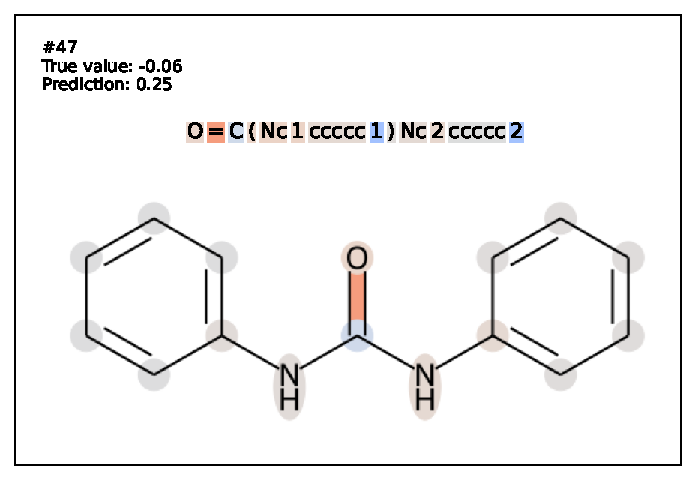
\includegraphics[width=\textwidth]{figures/esol/esol47.pdf} 
\end{subfigure}
\begin{subfigure}[b]{0.33\textwidth} 
  \centering 
  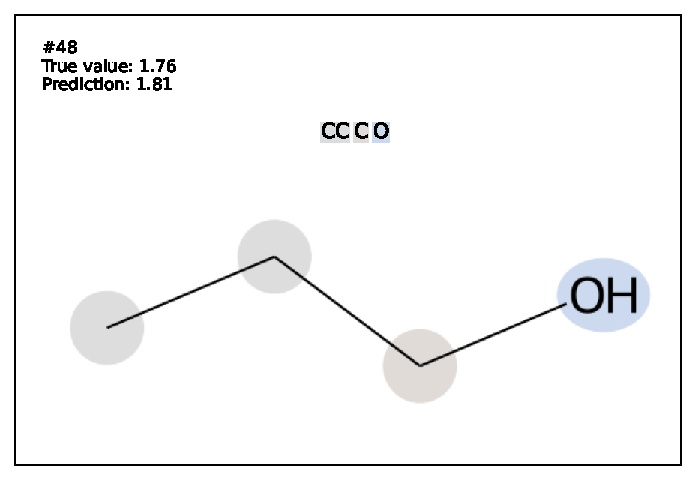
\includegraphics[width=\textwidth]{figures/esol/esol48.pdf} 
\end{subfigure}\begin{subfigure}[b]{0.33\textwidth} 
  \centering 
  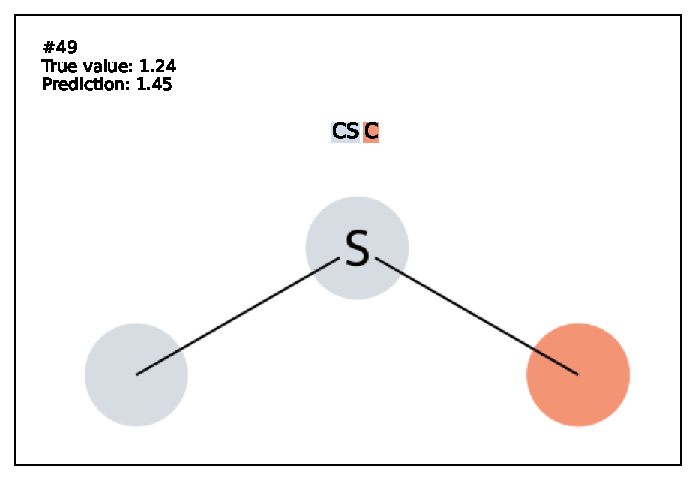
\includegraphics[width=\textwidth]{figures/esol/esol49.pdf} 
\end{subfigure}\begin{subfigure}[b]{0.33\textwidth} 
  \centering 
  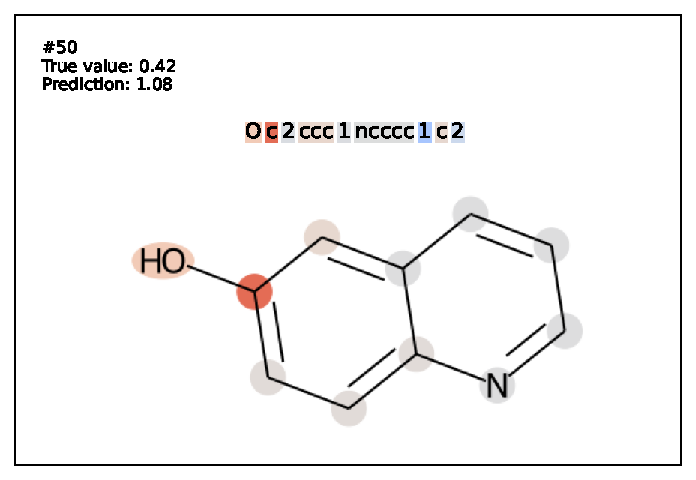
\includegraphics[width=\textwidth]{figures/esol/esol50.pdf} 
\end{subfigure}
\begin{subfigure}[b]{0.33\textwidth} 
  \centering 
  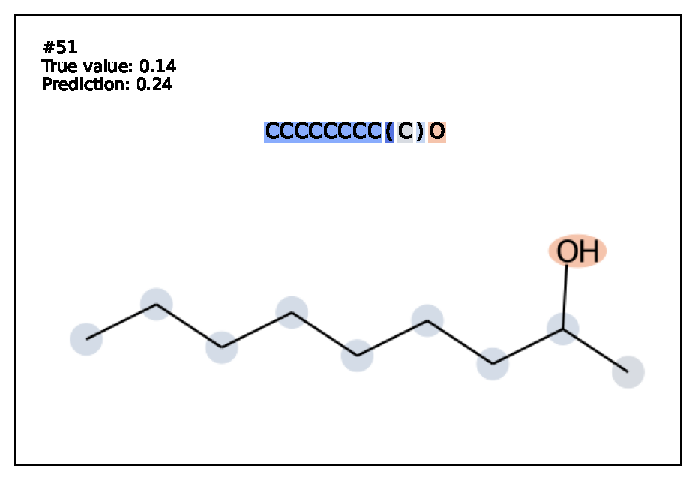
\includegraphics[width=\textwidth]{figures/esol/esol51.pdf} 
\end{subfigure}\begin{subfigure}[b]{0.33\textwidth} 
  \centering 
  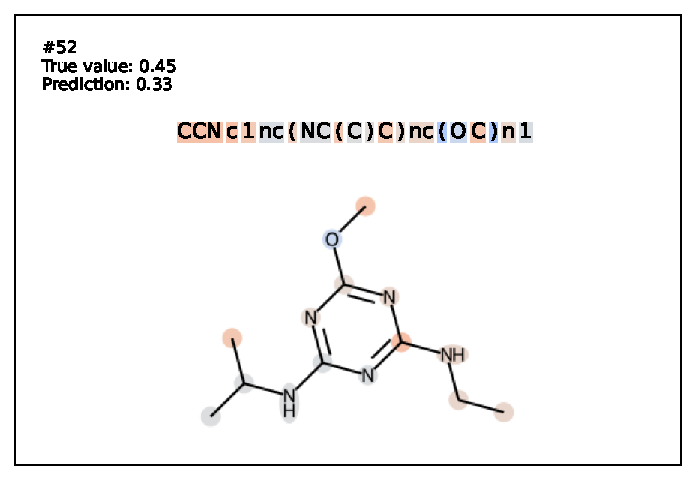
\includegraphics[width=\textwidth]{figures/esol/esol52.pdf} 
\end{subfigure}\begin{subfigure}[b]{0.33\textwidth} 
  \centering 
  \includegraphics[width=\textwidth]{figures/esol/esol53.pdf} 
\end{subfigure}
\begin{subfigure}[b]{0.33\textwidth} 
  \centering 
  \includegraphics[width=\textwidth]{figures/esol/esol55.pdf} 
\end{subfigure}\begin{subfigure}[b]{0.33\textwidth} 
  \centering 
  \includegraphics[width=\textwidth]{figures/esol/esol56.pdf} 
\end{subfigure}\begin{subfigure}[b]{0.33\textwidth} 
  \centering 
  \includegraphics[width=\textwidth]{figures/esol/esol57.pdf} 
\end{subfigure}
\begin{subfigure}[b]{0.33\textwidth} 
  \centering 
  \includegraphics[width=\textwidth]{figures/esol/esol58.pdf} 
\end{subfigure}\begin{subfigure}[b]{0.33\textwidth} 
  \centering 
  \includegraphics[width=\textwidth]{figures/esol/esol59.pdf} 
\end{subfigure}\begin{subfigure}[b]{0.33\textwidth} 
  \centering 
  \includegraphics[width=\textwidth]{figures/esol/esol60.pdf} 
\end{subfigure}


\caption{Explaining predictions of the fine-tuned model on ESOL dataset. See Section \ref{sec:captum}. Part 3/3}
\label{fig:captum-esol-3}
\end{figure}

In \Cref{fig:captum-esol-1,fig:captum-esol-2,fig:captum-esol-3} we show the attributions on $60$ molecules from the test set of ESOL dataset. The images with indices 10, 16, 19, 27, 30, 37, 50, 51 and 55 contain hydroxyl groups, which are properly highlighted in red by the Integrated Gradient method. Same with carbonyl groups, as seen on molecules with indices 2, 5, 7, 12,%
25, 26, 46 and 47.



It is usually assumed that the noise in aqueous solubility datasets is roughly 0.7 \citet{ml-solubility-noise}. It is noteworthy that in all instances, the errors of the predicted values are less than that and, hence, can be assumed to be accurate. %

In one case, out of all molecules bearing the hydroxyl group, in compound \#48, the functional group was not highlighted and even marked as a negative contributor. Even so, the prediction value of solubility was correct. 

One more interesting example where the hydroxyl group has been recognized, but the prediction was incorrect (LogS ± 0.76) is compound \#34. In this compound, in addition to the hydroxyl group, four alkyl chloride (C-Cl) groups exist and contribute to the molecule's solubility (have a lower level of polarity). The lower proportion of alkyl chloride-bearing compounds in the training set may lead to underestimating these functional group contributions to the molecule's solubility. 

In the case of carbonyl groups, there are more examples where the Integrated Gradients method didn't highlight the functional groups, for instance, compounds under the numbers 13, 14, 17, 35, 36, 40, 41, 42 and 43. Note that logS values of all these compounds were in the range of 0 to $-2$, which is the range of less soluble compounds, compared to the solubility of aforementioned compounds with recognized carbonyl groups (in the range of 0 and higher, highly soluble).
Additionally, all compounds with unrecognized carbonyl groups are complex, polycyclic aromatic hydrocarbons, which, as mentioned in the Ames dataset, was more problematic for the analysis by the Integrated Gradients method. 


Other interesting examples are in the aliphatic compounds, which are hydrocarbon compounds containing carbon and hydrogen joined together in straight chains with carbonyl groups (Compounds \# 7, 25, 26, 28) or hydroxyl groups (Compounds \# 19, 48, 51). A general rule for these compounds is that the longer the carbon chain, the lower the solubility in polar solvents such as water. Here, we see that the increasing amount of CH2 groups in a carbon chain enhances the hydrophobic effect, which decreases the solubility value. Hence, compounds \#28 and \#51 have the lowest solubility compared to the abovementioned examples. It is remarkable that the model somehow followed the rule, and predicted values also exhibit the same pattern. As to the Integrated Gradients method, the negative contribution of CH2 groups is constantly highlighted in all compounds, whereas peripheric CH2 groups have been marked as small contributions to solubility. 

There are other examples where the predictions were accurate, but the underlying chemistry is more complicated, and the highlighted substructures sometimes are unexplainable. 